
\section{Présentation}
Le banc de test correspond au système composé du capteur et des appareils des mesures. Pour ce banc de test, le matériel suivant est utilisé :
\begin{itemize}
    \item Capteur avec son support (Design 1 ou 5)
    \item Débitmètre de référence FESTO SFAH
    \item Electrovanne FESTO
    \item Arduino Nano
    \item transistor MOSFET IRL540N
\end{itemize}

Le débitmètre de référence est un débitmètre FESTO bidirectionnel dont la datasheet se trouve en annexe. Son graphe de calibation  a été
construit grâce à la sortie analogique fournie par le débitmètre :
\begin{figure}[H]
    \centering
    \includegraphics[scale = 0.4]{assets/figures/Calibration_maison.jpg}
    \caption{Tension en fonction du débit}
    \label{fig:calibration}
\end{figure}

Sur le figure \ref{fig:calibration}, nous pouvons observer la tension mesurée en fonction d'un certain débit d'air. Les paramètres utilisés
pour cette calibration sont les suivants :
\begin{itemize}
    \item Sortie analogique en tension sur une plage de 0V à 10V
    \item Full Scale allant de 0\% à +100\%
\end{itemize}

Le graphe montre une fonction linéaire qui se rapproche très fortement de la fonction $y = x$ (f$_{mesur\acute{e}}$(x) = 1.0004x - 0.0038).

\section{Catalogue des solutions}
\subsection{Flux d'air pulsé}
Une première solution est d'amener un flux d'air pulsé sur la membrane. Ce flux d'air serait contrôlé par une électrovanne et un
transistor MOSFET IRL540N. Ce transistor a été choisi car il permet d'être contrôlé grâce à un Arduino Nano. En effet, sa tension de seuil
($V_{GS}$) est de 4V, 5V ou 10V. Etant donné que l'Arduino Nano sortira une tension de 5V, cette valeur sera suffisante pour faire fonctionner
le MOSFET.
\begin{figure}[H]
    \centering
    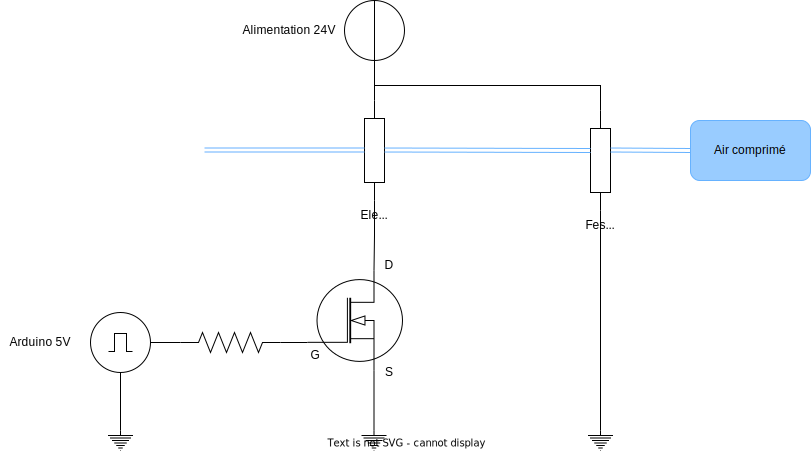
\includegraphics[scale=0.6]{assets/figures/MOSFET.png}
    \caption{Schéma électrique avec MOSFET}
    \label{fig:MOSFET}
\end{figure}
Un contrôle de la chaleur dégagée par effet Joule est utile afin de décider si un dissipateur thermique est nécessaire. Ce calcul se fait
de la manière suivante :\\
D'abord, calculons la chaleur dégagée (puissance par effet Joule) :

\[I_{electrovanne} = \frac{P_{electrovanne}}{U} = \frac{6.5}{24} \cong 0.27 A \]
\[P_{effetJoule} = R_{DS}\cdot I^2\]
Avec :\\
$R_{DS}$ (résistance entre les jonctions D et S du MOSFET) = 0.053

\begin{equation}
    P_{effetJoule} = 0.053\cdot 0.27^2 \cong 3.86mW
\end{equation}

Les différentes valeurs de résistances, puissances, etc. se trouvent dans la datasheet du MOSFET qui se trouve en annexe. \\

Puis, nous pouvons calculer la puissance maximum dissipée par le MOSFET :
\[P_{max\,dissip\acute{e}e} = \frac{max(T_j) - T_A}{R_{\theta JA}} = \frac{175-25}{62}\cong 2.42 W\]
Avec :\\
$T_j$ = température de jonction\\
$T_A$ = température ambiante\\
$R_{\theta JA}$ = résistance thermique, de jonction à ambiant

Ainsi, comme $P_{effetJoule} < P_{max\,dissip\acute{e}e}$, un dissipateur thermique n'est pas nécessaire. \\

Au niveau du fonctionnement général du système, le transistor est commandé par un Arduino Nano qui alimente le MOSFET avec 5V par pulsation (1 seconde à 5V et 1 seconde à 0V). \\
Lorsque le MOSFET reçoit 5V, il s'active et "laisse passer" le courant qui permet à l'électrovanne de s'ouvrir et de faire passer le
flux d'air.
\begin{figure}[H]
    \centering
    \begin{subfigure}[b]{0.45\textwidth}
        \hspace{-1.5cm}
        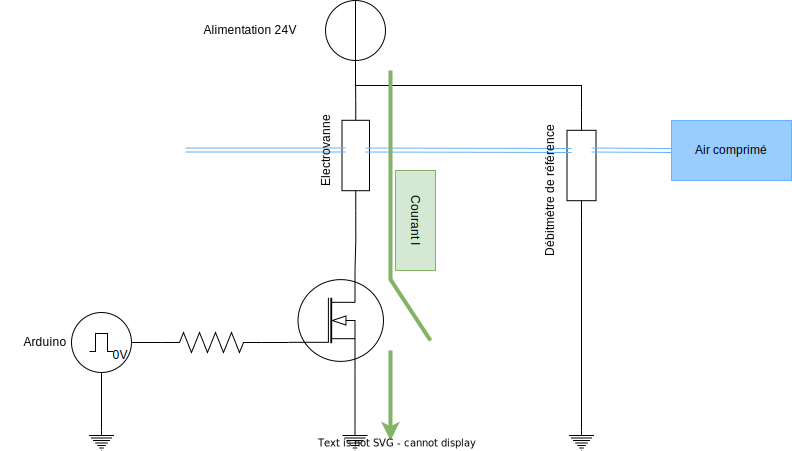
\includegraphics[scale = 0.3]{assets/figures/MOSFET_0V.png}
        \caption{MOSFET non-alimenté}
        \label{fig:MOSFET_0V}
    \end{subfigure}
    \begin{subfigure}[b]{0.45\textwidth}
        \centering
        \includegraphics[scale = 0.3]{assets/figures/MOSFET_5V.png}
        \caption{MOSFET alimenté}
        \label{fig:MOSFET_5V}
    \end{subfigure}
    \caption{Fonctionnement du flux d'air pulsé}
    \label{fig:flux_pulse}
\end{figure}

Le corps de chauffe, constitué d'une fine couche d'or, doit être alimenté avec un certain courant. Ce courant, s'il est trop élevé, va abîmer la
membrane mais s'il est trop bas, il sera insuffisant pour entraîner une différence de température de part et d'autres du capteur. \\

Le calcul suivant a don été effectué afin de déterminer le courant à utiliser pour le corps de chauffe :
\[P_{max} = R\cdot I^2\]
Avec :\\
$P_{parSurface}$ (puissance max par unité de surface) = 100 $\frac{W}{m^2}$\\
$R$ (résistance du corps de chauffe) = 45 $\Omega$\\

La valeur de puissance par unité de surface a été tirée de la puissance maximale utilisée pour les chauffages du marché (chauffage au sol).
Elle permet d'avoir un ordre de grandeur pour la valeur de courant à fournir au corps de chauffe.
La surface du corps de chauffe à été approximée à 80 mm$^2$ ($2mm x 40mm$).\\
Ainsi une règle de 3 a été effectuée afin de trouver la valeur de puissance pour le corps de chauffe concerné :
\[P_{max} = 8\cdot 10^{-5}\cdot 100 = 1.78\cdot 10^{-4}\]
\[I = \sqrt{\frac{P_{max}}{R}} = \sqrt{\frac{1.78\cdot 10^{-4}}{45}} \cong 13 mA\]
Plusieurs tests ont été alors effectué dans une plage de 10 mA à 20 mA. Ces tests ont donné un courant maximum a 15 mA. Au-delà, la membrane
est abîmée (couche d'or rongée).

\subsection{Corps de chauffe pulsé}

\section{Validation}
